\chapter{Simulation Study 1}
\label{C:chap_sim2}


This Simulation study is based strongly on \cite{Morden2011} with the major innovation being to induce a correlation between time to progression (TTP) and overall survival (OS) when generating the survival times.  In this simulation study I have two major objectives. Objective 1 is to confirm the results of \cite{Morden2011} once the correlations between endpoints discussed in Section \ref{S:chap_intro:correlation} are introduced. Objective 2 is to investigate the sensitivity of the rank preserving structural failure time method to variations in implementation. 

\section{Scenarios Assessed}



\subsection{Summary of Simulation Parameters}

Table \ref{T:chap_sim2:sim1parm} shows a summary of the scenarios investigated and chosen parameters. For each of the 9 basis scenarios investigated $\rho$, the correlation between Time to Progression and Overall Survival, is varied across 6 levels leading to 54 scenarios in total. For each of these 54 scenarios 1000 datasets are simulated. For this simulation the reduction in hazard due to treatment is considered to be the same during and after experimental treatment with switch patients receiving the same effect as randomized patients.

\begin{table}[ht] 
\caption{Summary of parameters for simulation study 1}
\centering 
\begin{tabular}{ l l l }
\hline
\hline
Parameter & Description & Values \\
\hline
$\exp(\beta_{1a})$        & Treatment Effect on overall survival & $0.7$, $0.9$, $1.0$ \\
                          & with $\beta_{1b}=\beta_{2a}=\beta_{2b}$    &                     \\
\hline                          
$p_{\verb+SWITCH+}$ & Proportion of control arm who switch &  $0.2$, $0.4$, $0.6$ \\
\hline
$\rho$                    & Correlation between TTP and OS  &  $0$, $0.2$, $0.4$, $0.6$, $0.8$ \\
\hline 
\end{tabular} 
\label{T:chap_sim2:sim1parm}
\end{table}


\section{Methods assessed}
\label{S:chap_sim2:methass}
Of the adjustment methods described in Chapter \ref{CHAP:methods} only a selection are assessed here. 
\subsection{Simple methods}
To estimate a Hazard ratio using simple methods the following approaches are taken.
\begin{itemize}
\item Intention-to-treat (ITT) - A Cox model will be fit to the observed data with no adjustment for treatment switching. 
\item Per-protocol Excluding Switch Patients (PP-EX) - A Cox model will be fit to the observed data excluding patients who switch.
\item Per-protocol Censoring at Switch (PP-CENS) - A Cox model will be fit to the observed data censoring patients who switch at the time of their switch.
\item Treatment as a time-varying covariate (TVC) - A Cox model will be fit to the observed data including a covariate for experimental therapy that is time dependent.
\item Switch Treatment as a time-varying covariate (TVC2) - A Cox model will be fit to the observed data including
a covariate for randomized treatment and a second covariate for switch therapy that is time dependent.
\end{itemize}
\subsection{Complex Methods}
\subsubsection{modified Iterative Parameter Estimation (MIPE)}
The IPE method including the modified re-censoring algorithm of \cite{Zhang2016} will be used as discussed in Section \ref{S:chap_methrev:MIPE}. Two approaches will be used to derive a Hazard Ratio the first will be to do a comparison of Observed ($T_i$) for experimental and Latent ($U_i$) for control survival times labelled as MIPE. The second will be to use the dual accelerated failure time and proportional hazards nature of the Weibull distribution to apply Equation \ref{E:chap_sim2:mipehr} where $\eta$ is the treatment effect estimated by Weibull regression and $\gamma$ is the shape parameter of this regression at convergence of the procedure (MIPE-WEIB). 

\begin{equation}
\label{E:chap_sim2:mipehr}
\beta = -\eta\gamma
\end{equation}

\subsection{Two-stage AFT}
To apply the two-stage AFT method it is necessary to define a secondary baseline. In this simulation the only switching that occurs is at time of progression so this is the natural choice. It is also necessary to consider any covariates that could affect survival separately to treatment at this second baseline. In this simulation no such covariates exist, however, as time to progression is correlated with overall survival this could potentially lead to situations where time to progression is predictive of the length of survival post progression. As such two AFT models will be investigated in the application of this method. In the first model the time to progression is included as a covariate (2SAFT) while for the second model is the null model where no covariates are included (2SAFT-NULL). As discussed in Section \ref{S:chap_meth:2saftcens} the recensoring algorithm described by \cite{Latimer2016} may censor more events than needed so additionally both these models will be implemented without re-censoring (labelled as NC in the results).

\subsubsection{Rank preserving-structural failure time (RPSFT) models} 
Six variations of RPSFT will be assessed in this simulation study. The first variation is the choice of test used in the g-estimation as discussed in Section \ref{S:chap_methrev:RPSFTfit} where I will investigate the use of both log-rank test and wilcoxon test. The second variation involves the choice of the ``treatment group'' or ``on treatment'' model as discussed in Section \ref{S:chap_methrev:RPSFTonep} where time on treatment will be taken to be the duration of progression free survival. The final variation was to investigate whether re-censoring of the experimental therapy arm prior to calculation of a counter-factual Hazard Ratio has in impact on the results as discussed in Section \ref{S:chap_methrev:RPSFTestHR}. The combination of these variations is detailed in Table \ref{T:chap_sim2:Sim1RPSFTlab} alongside the Label used to identify these approaches in the results. For the ``on treatment'' analysis the duration of experimental therapy will be assumed to have been the time to progression for first line ($T_{PD}$) or for second line ($T_{PD_2}-T_{PD}$) as discussed in Chapter \ref{C:chap_sim_design}. 

\begin{table}[ht] 
\caption{Approaches to RPSFT investigated in simulation study 1}
\centering 

\begin{tabular}{ l c c c}
\hline
\hline
Label  & g-estimation     & Modelling  & Comparison used            \\
       & test             & approach   & to estimate                \\
       &                  &            & Hazard Ratio               \\ 
\hline 
RPSFT-TG-LR    & log-rank & ``treatment group'' & $T_i$ vs $U_i$ \\
RPSFT-OT-LR-TU & log-rank & ``on treatment''    & $T_i$ vs $U_i$ \\
RPSFT-OT-LR-V  & log-rank & ``on treatment''    & $V_i$ vs $V_i$ \\
\hline
RPSFT-TG-W     & Wilcoxon & ``treatment group'' & $T_i$ vs $U_i$ \\
RPSFT-OT-W-TU  & Wilcoxon & ``on treatment''    & $T_i$ vs $U_i$ \\
RPSFT-OT-W-VV  & Wilcoxon & ``on treatment''    & $V_i$ vs $V_i$ \\
\hline 
\end{tabular} 
\label{T:chap_sim2:Sim1RPSFTlab}
\end{table}


\subsubsection{Convergence of complex methods}

\label{S:chap_sim2:convimp}

For both the RPSFT and MIPE methods it is possible that they will not converge to a unique value of $\psi$ and $\eta$ respectively. For both methods proposals have been made to derive a unique solution in  these cases. For MIPE \cite{Zhang2016} propose taking the mean of the last 20 estimates of the MIPE procedure, while for RPSFT \cite{White1999} describes a weighted mean of estimates as discussed in Section \ref{S:chap_methrev:ESTissues}. The analysis with these imputations applied have the results labelled by the suffix -ALL.

\section{Results}
\label{S:chap_sim2:resmeth}

For this simulaton study the primary outcome being assessed is the Hazard Ratio for overall survival. This is assessed by considering the mean Hazard Ratio ($\hat{\exp(\beta)}$), bias and mean square error (MSE) calculated using the methods of \cite{Burton2006}. The coverage is estimated as the proportion of simulations for a scenario where the estimated 95\% confidence intervals contained the true value Hazard Ratio.

Table \ref{T:chap_sim2:simres} shows the range of results by method and true Hazard Ratio seen across the range of scenarios considered in this simulation study. As the results for the RPSFT method using the wilcoxon test were very similar to those using the log-rank test they are not presented here but can be found in Appendix \ref{A:sim2res} along with complete results for each scenario in this study. 

\begin{table}[ht] 
\caption{The range of bias, MSE, coverage and convergence across all scenarios}
\centering 
% latex table generated in R 3.3.1 by xtable 1.8-2 package
% Thu Sep 15 18:20:51 2016
\scalebox{0.9}{
\begin{tabular}{lrrrr}
  \hline
\hline
Method & Bias  & MSE & Coverage & Convergence  \\   & $(\%)$ &   & $(\%)$ & $(\%)$ \\   & min, max & min, max & min, max & min, max \\ 
  \hline
ITT &   0.04, 20.45 & 0.01, 0.04 & 76.8, 96.7 & 100.0, 100.0 \\ 
  PP-CENS &   0.15, 50.14 & 0.01, 0.32 & 40.4, 96.3 & 100.0, 100.0 \\ 
  PP-EX & -34.09,  4.66 & 0.01, 0.13 & 23.8, 96.0 & 100.0, 100.0 \\ 
  TVC &   0.10, 79.81 & 0.01, 0.72 &  3.7, 96.1 & 100.0, 100.0 \\ 
  TVC2 &   0.14, 59.00 & 0.01, 0.42 & 24.7, 96.5 & 100.0, 100.0 \\ 
   \hline
RPSFT-TG-LR &  -0.48,  4.61 & 0.01, 0.07 & 91.0, 96.8 & 89.2, 100.0 \\ 
  RPSFT-TG-LR-ALL &   0.08,  6.23 & 0.01, 0.07 & 90.5, 96.7 & 100.0, 100.0 \\ 
   \hline
RPSFT-OT-LR-TU &   1.24, 24.90 & 0.02, 0.08 & 67.8, 96.9 & 20.5, 87.0 \\ 
  RPSFT-OT-LR-TU-ALL &  -4.64,  7.52 & 0.02, 0.07 & 82.9, 96.7 & 97.5, 100.0 \\ 
  RPSFT-OT-LR-V &  -2.88, 27.63 & 0.02, 0.17 & 82.0, 96.9 & 20.5, 87.0 \\ 
  RPSFT-OT-LR-V-ALL &  -9.63,  7.54 & 0.02, 0.16 & 85.3, 96.7 & 97.5, 100.0 \\ 
   \hline
2SAFT &  -0.34,  2.93 & 0.01, 0.03 & 85.3, 95.3 & 100.0, 100.0 \\ 
  2SAFT-NULL &   0.10,  3.75 & 0.01, 0.03 & 85.4, 95.0 & 100.0, 100.0 \\ 
  2SAFT-NC &   0.19,  3.73 & 0.01, 0.03 & 83.3, 95.7 & 100.0, 100.0 \\ 
  2SAFT-NC-NULL &   0.13,  6.74 & 0.01, 0.03 & 83.3, 95.7 & 100.0, 100.0 \\ 
   \hline
MIPE & -20.68, 10.45 & 0.03, 0.08 & 38.0, 90.0 & 24.8, 69.8 \\ 
  MIPE-ALL & -23.44, -1.91 & 0.03, 0.06 & 44.4, 82.0 & 100.0, 100.0 \\ 
  MIPE-WEIB &   1.47, 22.43 & 0.02, 0.09 &  & 24.8, 69.8 \\ 
   \hline
\end{tabular}
}

\label{T:chap_sim2:simres}
\end{table}


\subsection{Bias}
\subsubsection{Simple methods}
By considering Figure \ref{F:chap_sim2:simp_bias} it can be seen that for all the simple methods that the bias increases with a larger effect size and increasing proportion switching. For the ITT analysis the bias is not strongly related to the correlation between time to progression and overall survival and regardless of correlation this analysis underestimates the treatment effect as expected. When the effect size is large the bias reduces with increasing correlation this is likely due to the reduced exposure to experimental therapy in the control arm in these cases as suggested by Figure \ref{F:chap_sim_design:pfs_corr}. For the per-protocol analysis excluding switch patients (PP-EX) there is a large bias to overestimate the treatment effect regardless of correlation. 

For the per-protocol analysis censoring at crossover (PP-CENS) and both analysis using a cox model with time varying covariate (TVC and TVC2) it can be seen there are quite large levels of bias at all correlations and the level of bias is strongly dependent on the amount of correlation between time to progression and overall survival with these methods tending to underestimate the treatment effect when there is such a correlation. 

\begin{figure}[ht]
\centering
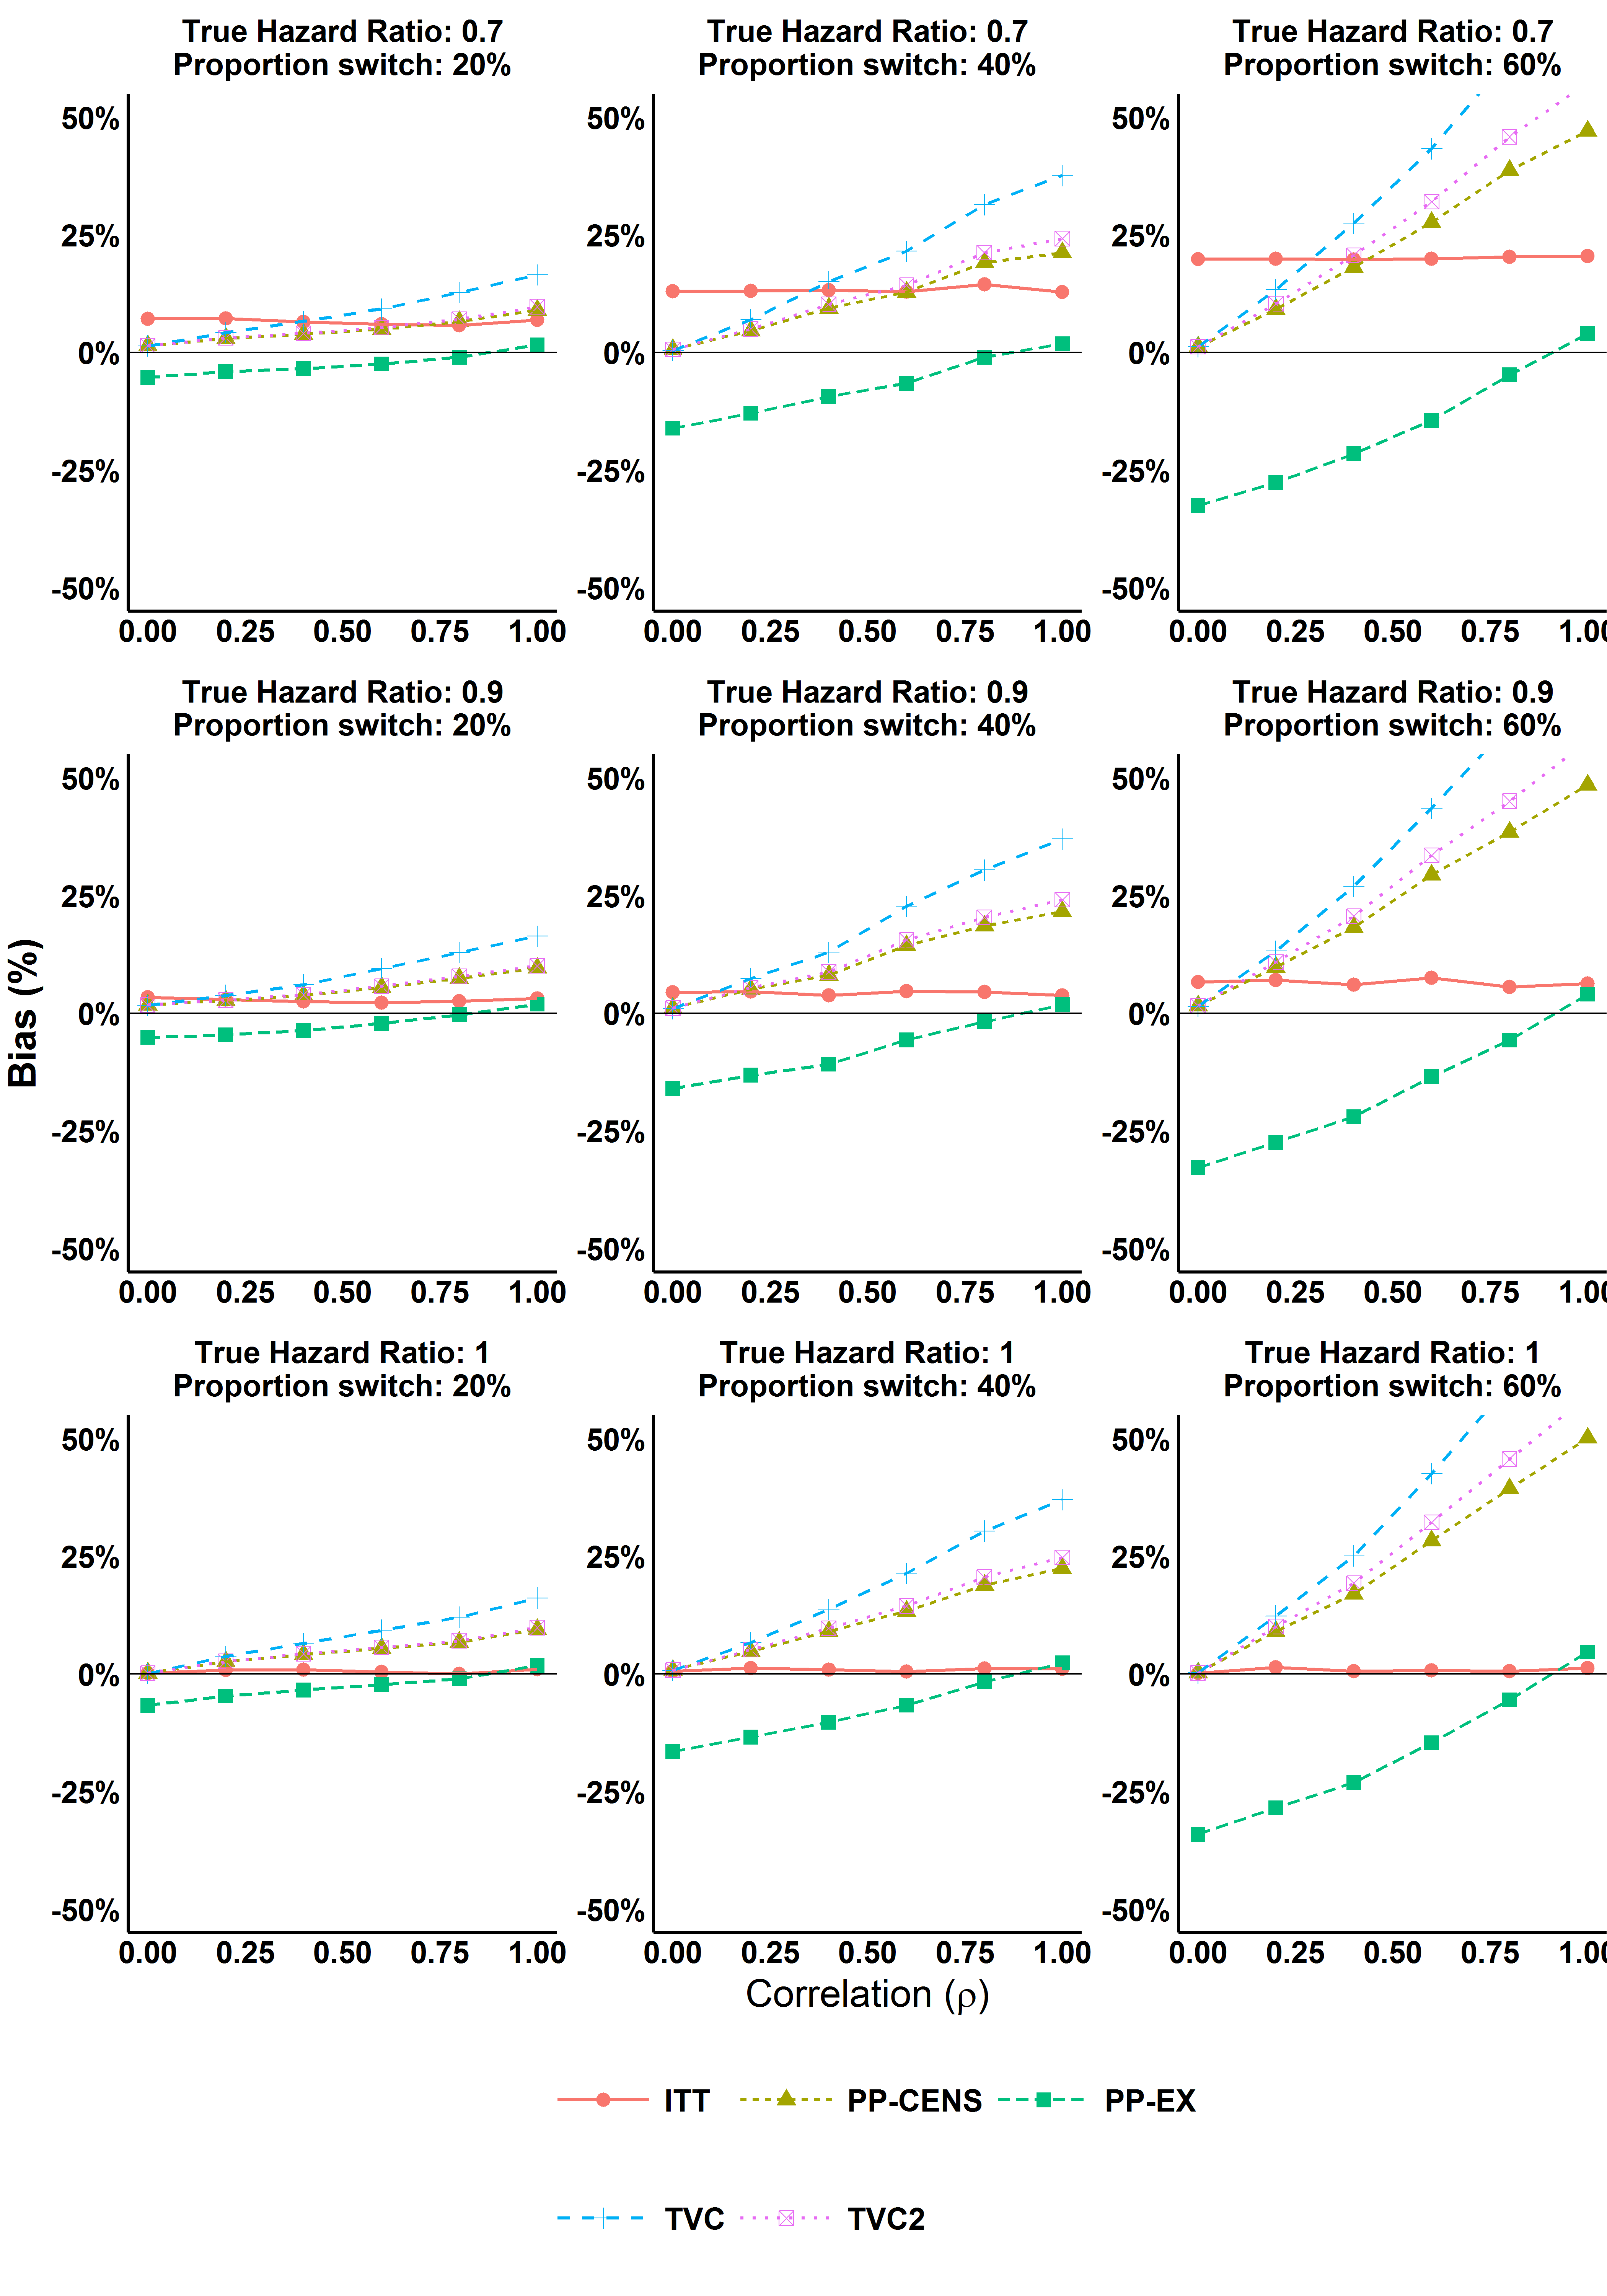
\includegraphics[width=13cm]{images/chap_sim2/simple_bias.png}
\caption{\label{F:chap_sim2:simp_bias} The bias for each of the simple methods across all the scenarios. It can be seen that the bias for ITT is mostly independent of correlation and tends to underestimate the treatment effect. For the Per-protocol Excluding Switch Patients (PP-EX) analysis the bias is large across all correlations and true hazard ratios once the proportion switch is greater than 20\%. For Per-protocol Censoring at Switch (PP-CENS) analysis and both analysis including Treatment as a time-varying covariate (TVC and TVC2) there is minimal bias when there is no correlation between survival and time to progression and very large bias otherwise. } 
\end{figure}

\subsubsection{Complex methods}

For the complex methods in these scenarios the correlation between Time To Progression and Overall Survival doesn't seem to much affect the bias observed as can be seen in Figure \ref{F:chap_sim2:comp_bias} and Figure \ref{F:chap_sim2:2saft_bias}. It can also be seen that the bias is much reduced compared to any of the simple methods regardless of scenario.

For the 6 variations of rank preserving survival time (RPSFT) models considered the choice of test log-rank (RPSFT-LR) or Wilcoxon (RPSFT-W) had negligible impact on the bias as can be seen in Appendix \ref{A:sim2res}. Considering the choice of modelling approach between ``treatment group'' (RPSFT-TG) and ``on treatment'' (RPSFT-OT) in general for this study it can be seen in Figure \ref{F:chap_sim2:comp_bias} the ``treatment group'' approach performed better though this is possibly because this better matches the way the data was generated. Of interest is that where the proportion switching is 40\% or less the ``on treatment'' modelling performs reasonably despite not matching the data generation procedure with bias < 0.05 across these scenarios. It can also be seen from this figure that the choice between estimating a hazard ratio from a comparison of observed and latent (RPSFT-OT-LR-TU) survival times or through using only counterfactual (RPSFT-OT-LR-V) times as discussed in Section \ref{S:chap_methrev:RPSFTestHR} has negligible impact.

For the modified iterative parameter estimation (MIPE) method in general bias was comparable to that of the RPSFT with estimation of the hazard ratio from the weibull parameters (MIPE-WEIB) generally having higher bias than when estimating the hazard ratio from a comparison of latent and observed survival times (MIPE). The exception is the scenarios with true Hazard Ratio of 0.7 and proportion switch of 20\% where it is unclear why the MIPE consistently underestimates the true Hazard Ratio regardless of correlation.

For the two-stage AFT approach the bias in absence of correlation is the same for all four models considered, however, once a correlation between time to progression and overall survival is introduced the model excluding PFS (2SAFT-NULL) has slightly increased bias. It also appears the omitting the recensoring algorithm increases the bias slightly.

\begin{figure}[ht]
\centering
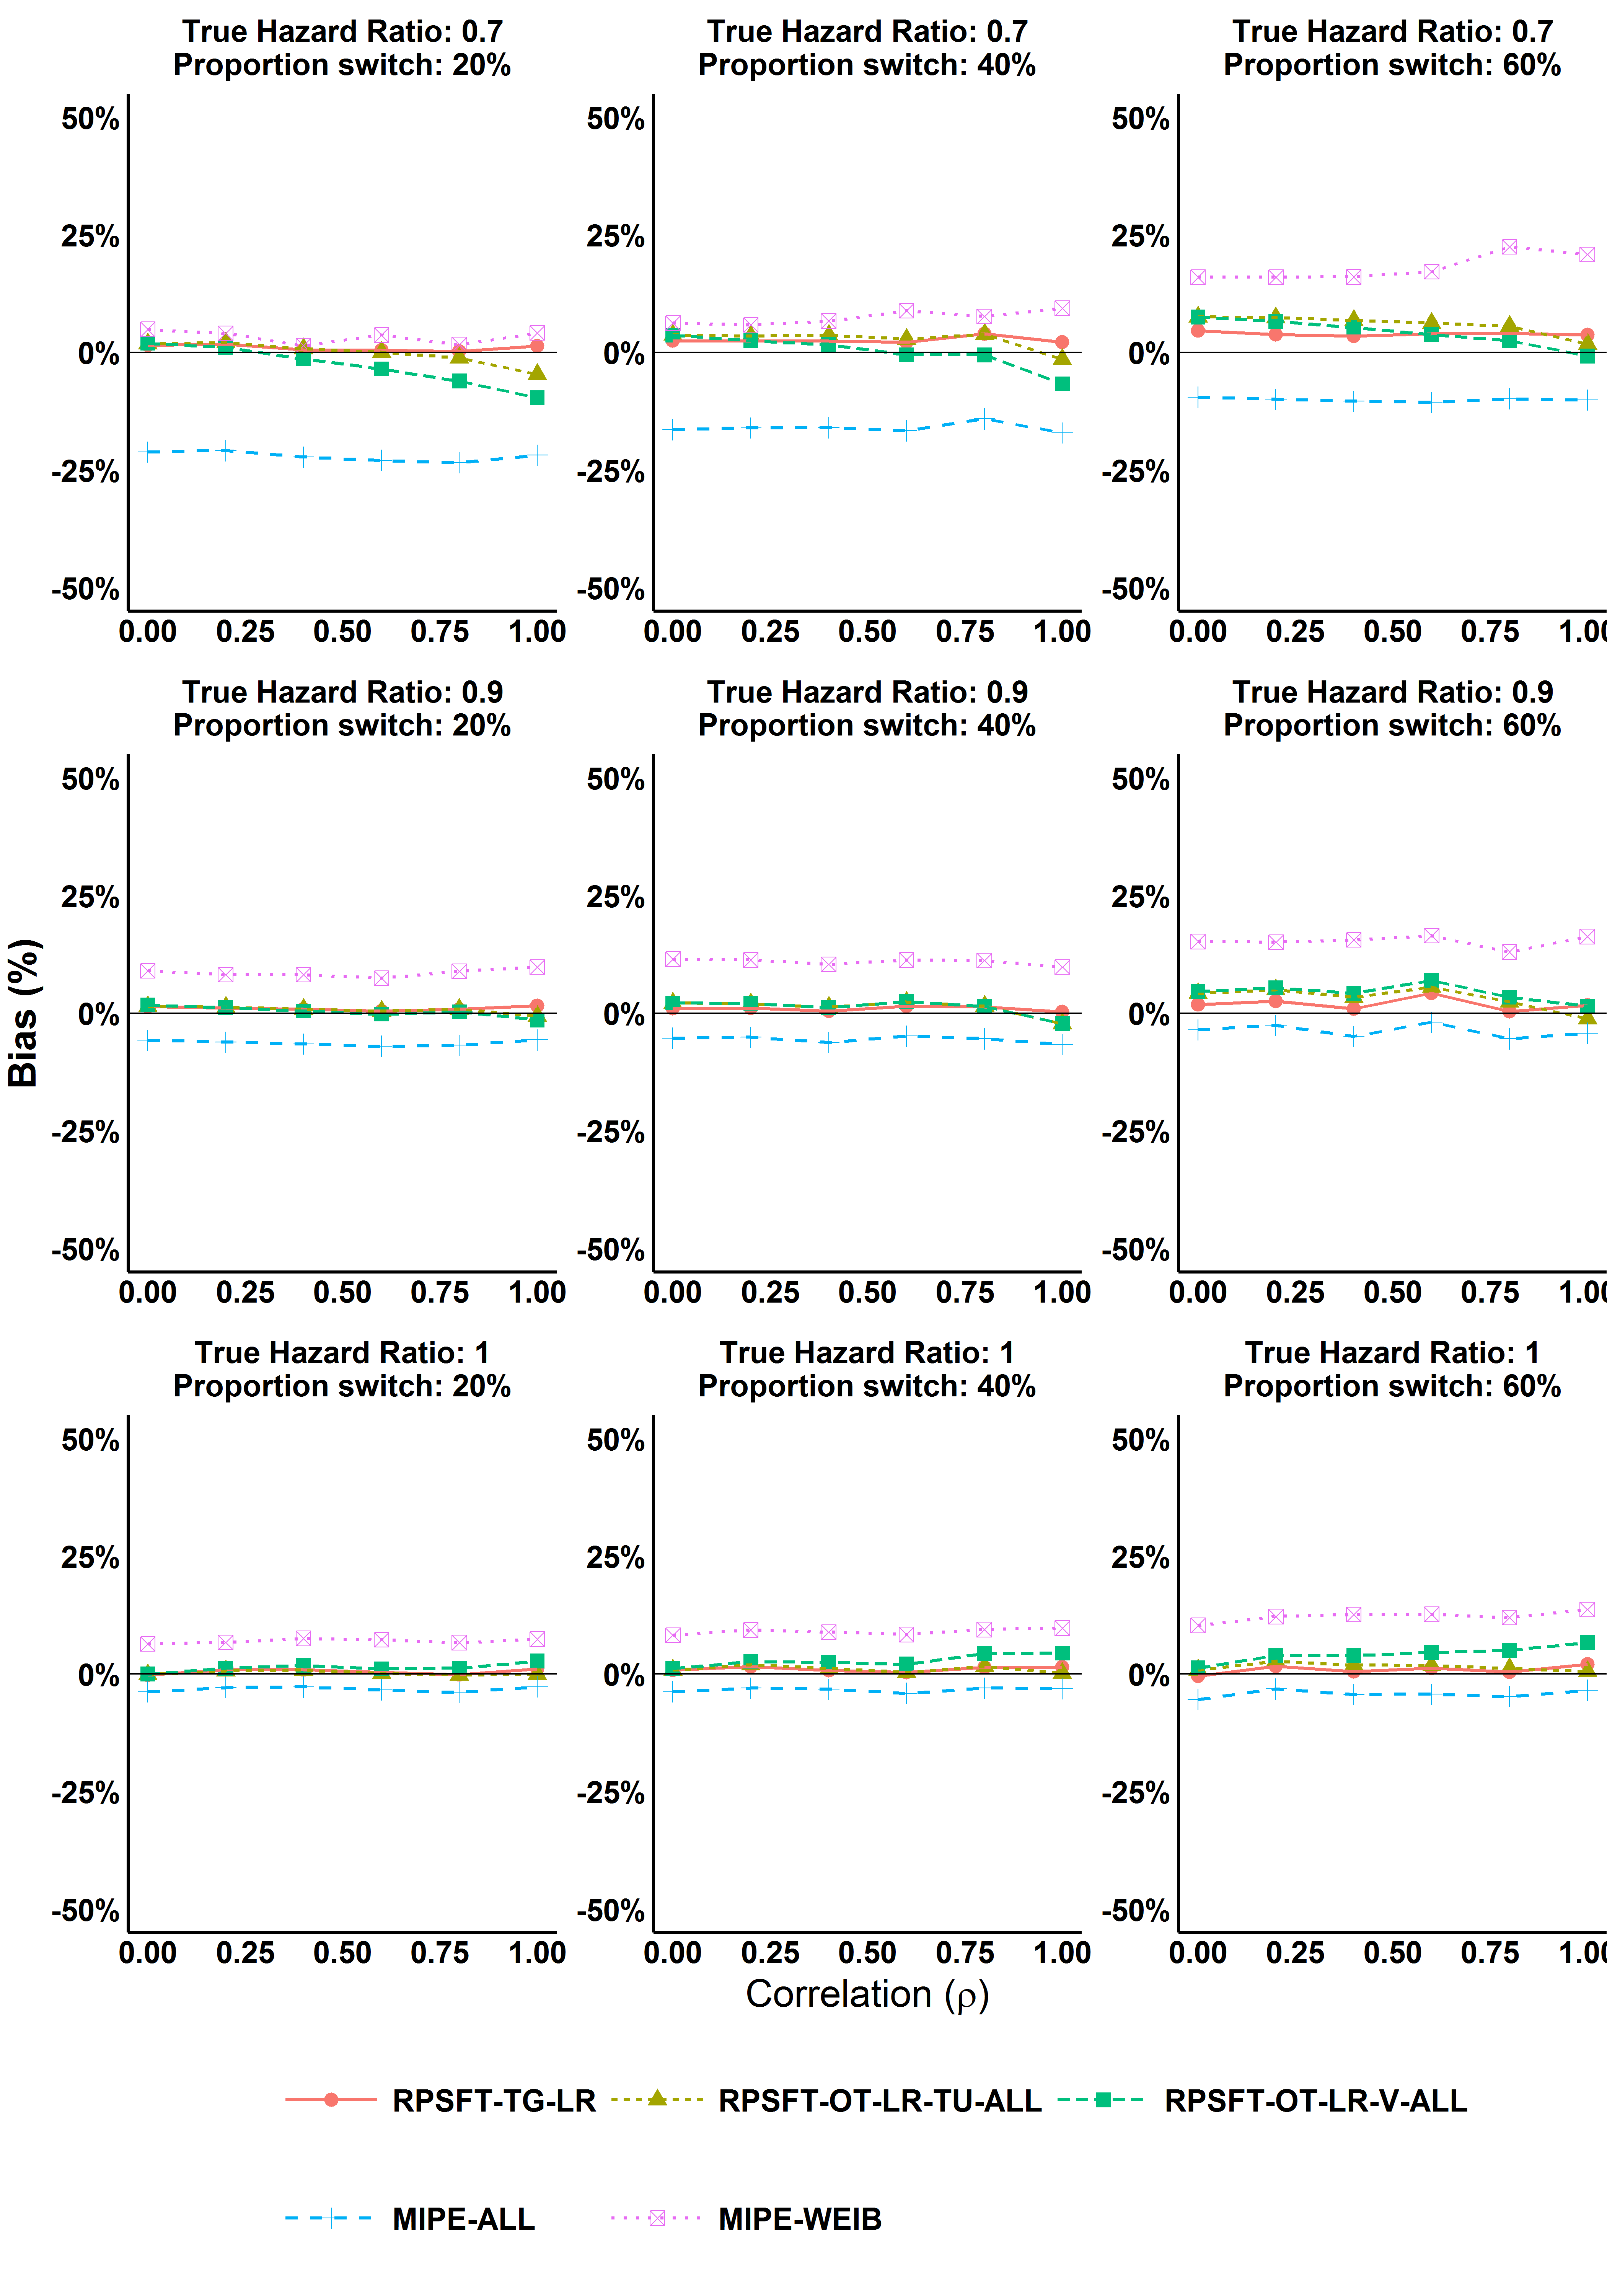
\includegraphics[width=13cm]{images/chap_sim2/complex_bias.png}
\caption{\label{F:chap_sim2:comp_bias} The bias for each of the complex methods across all the scenarios. Compared to the simple methods there is less relationship between correlation, proportion switch and bias. The bias of the Modified Iterative Parameter Estimation (MIPE) appears to depend on the method used to estimate the Hazard Ratio when the true treatment effect is large. For the three variations on RPSFT the absolute bias level is similar.} 
\end{figure}

\begin{figure}[ht]
\centering
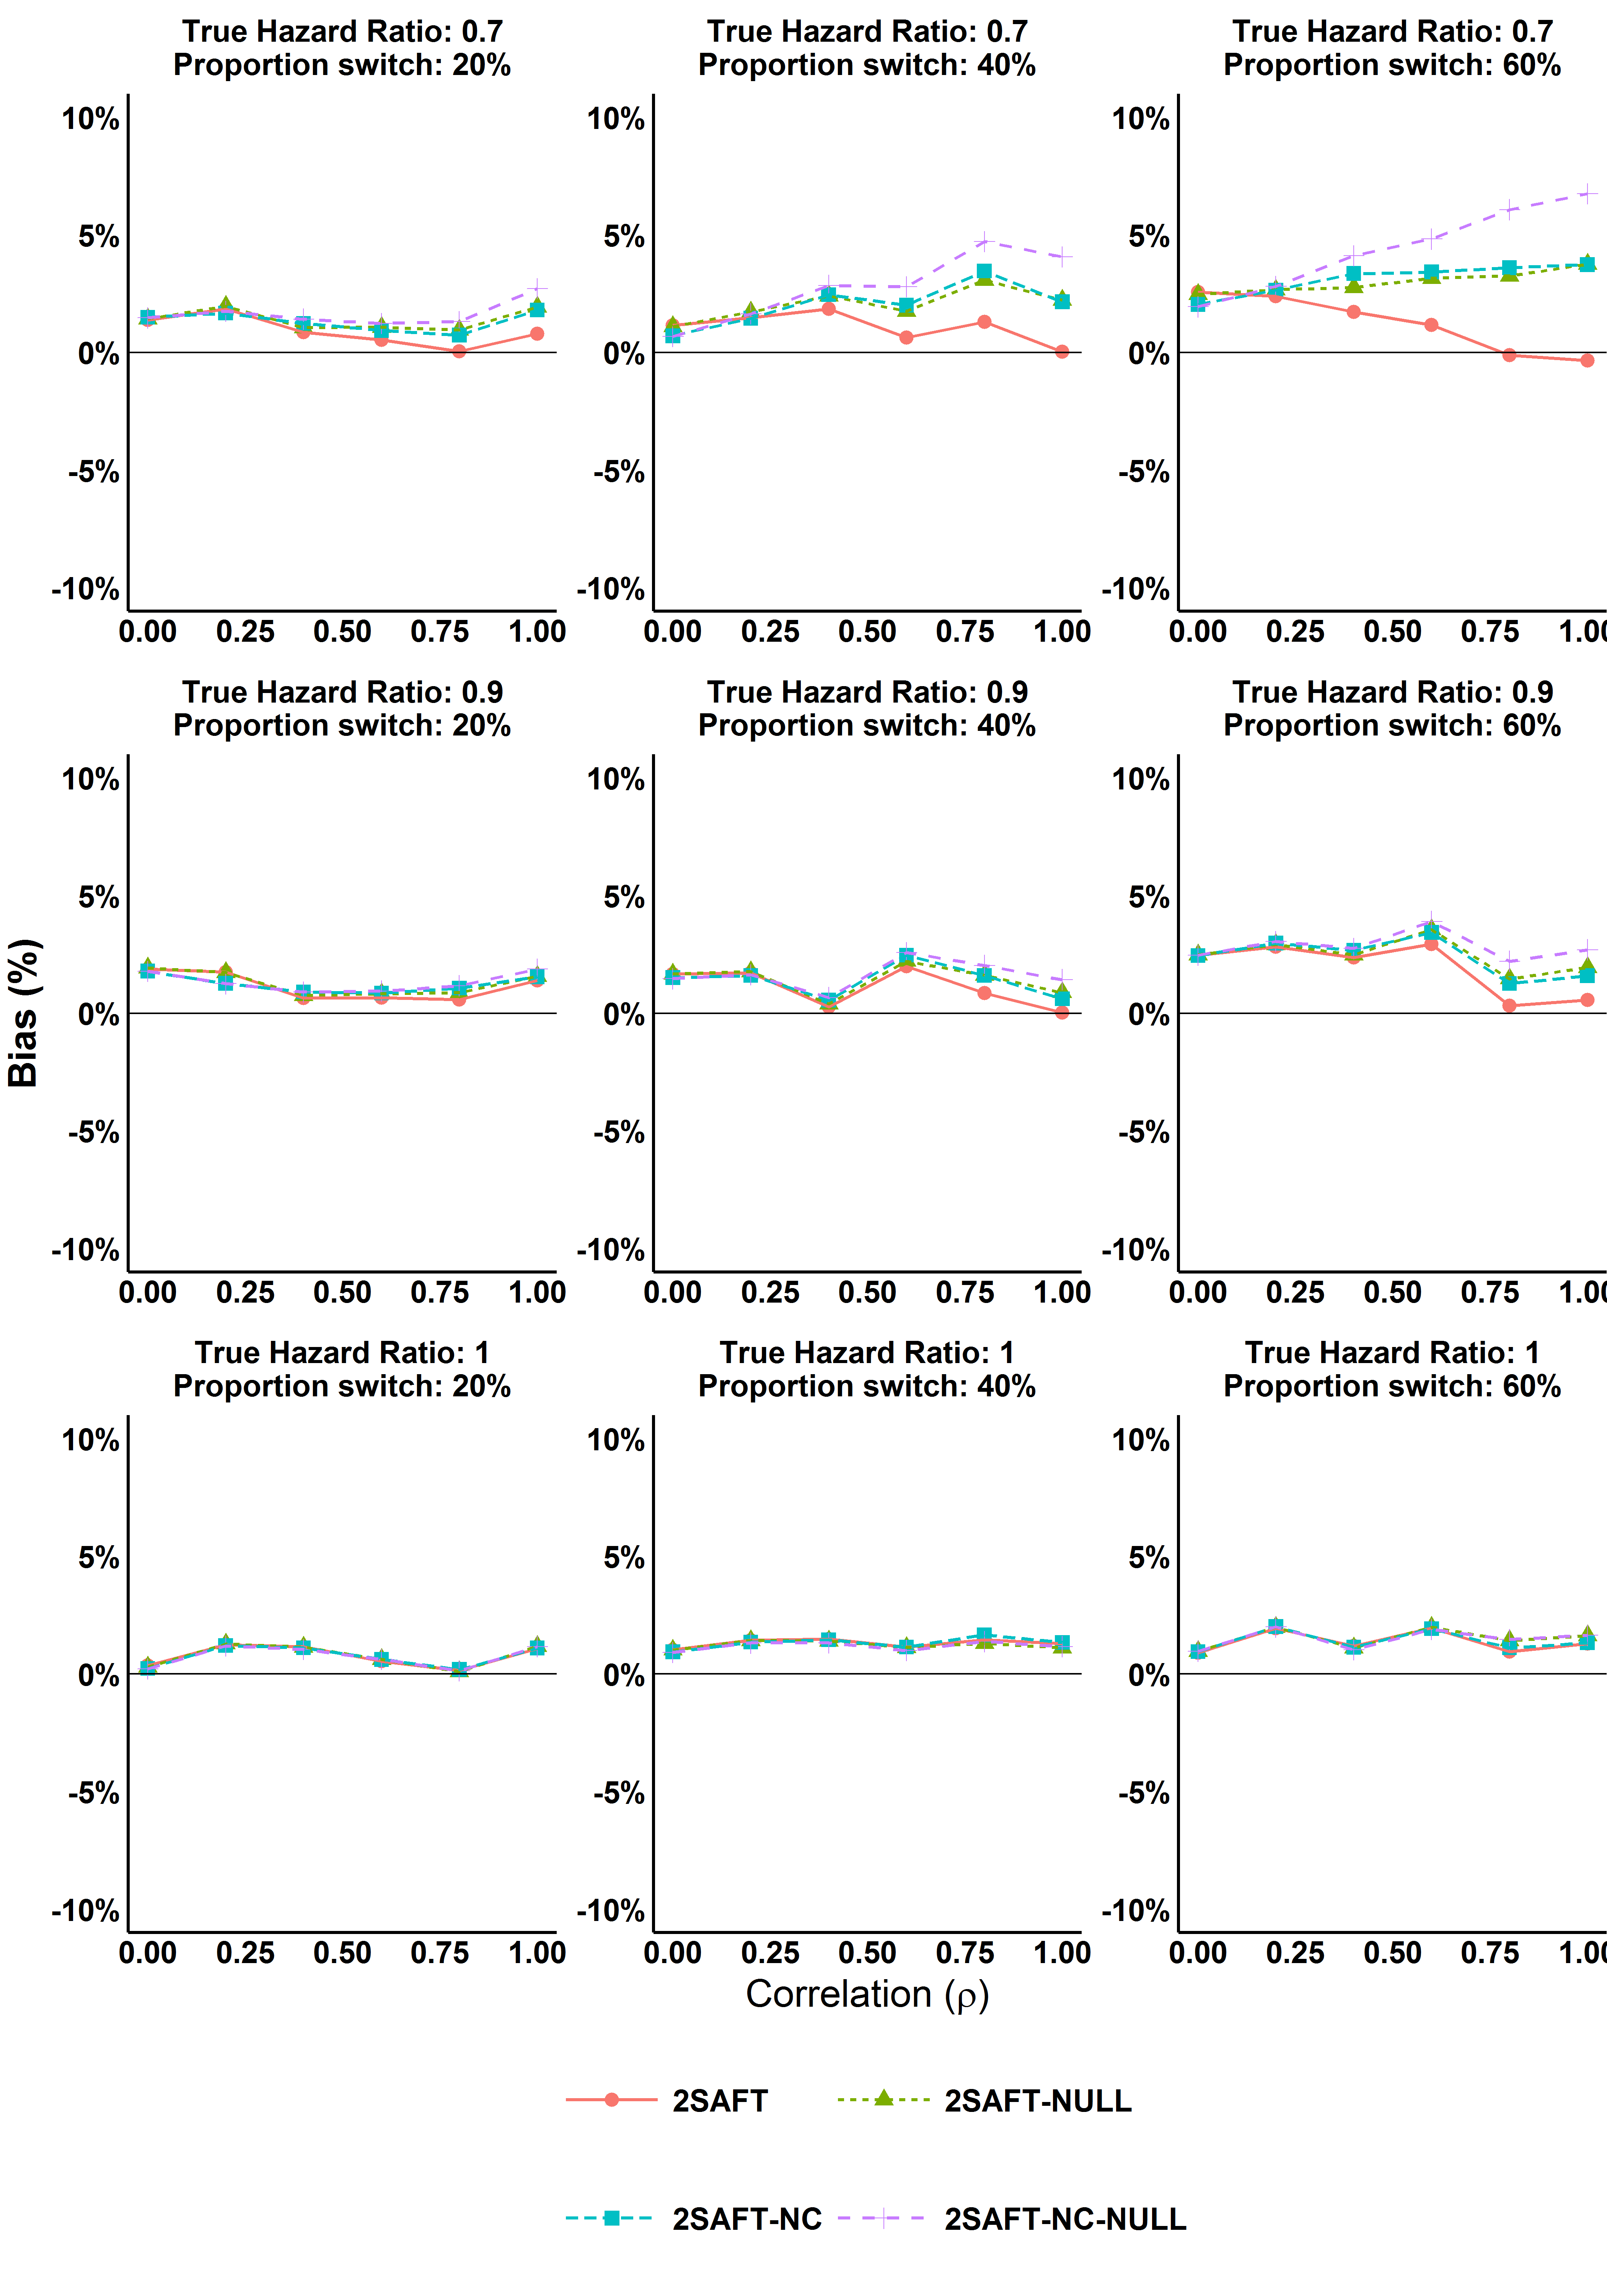
\includegraphics[width=13cm]{images/chap_sim2/2saft_bias.png}
\caption{\label{F:chap_sim2:2saft_bias} The bias for the various approaches to the two-stage AFT method across all the scenarios. The bias is low with no obvious relationship to correlation. NULL indicates that the model for survival post progression includes no covariates while NC indicates that no recensoring is implemented. For scenarios with larger treatment effect the importance of specifying the correct model and re-censoring is increased.} 
\end{figure}


\clearpage

\subsection{Coverage}

Figure \ref{F:chap_sim2:simp_cov} and Figure \ref{F:chap_sim2:comp_cov} show the coverage for the simple and complex methods respectively. It can be seen that the estimated confidence intervals from the Time varying covariate method (TVC) and per-protocol censoring at switch analysis (PP-CENS) have very poor coverage with even moderate levels of correlation. For the ITT method the lowest coverage is 76.8\% with coverage being worse with larger proportions of switching. When the true Hazard Ratio is 1.0 the coverage is stable between 93.9\% to 96.5\%.

For the per-protocol analysis excluding switchers (PP-EX) the coverage is poor across all scenarios and is often <50\% where the proportion who switch is 60\%.

For all the variations of RPSFT the 95\% confidence intervals are estimated using the correction described in Section \ref{S:chap_methrev:RPSFTestHR} and as can be seen in Table \ref{T:chap_sim2:simres} and Figure \ref{F:chap_sim2:comp_cov} the coverage for all scenarios is very stable for the ``treatment group'' (RPSFT-LR-TG) ranging from 90.5\% to 96.8\% across all 54 scenarios investigated. Similarly to the findings for bias the ``on treatment'' approach (RPSFT-LR-OT) tends to perform worse, however, the lowest coverage across all 54 scenarios was 82.0\% which is favourable compared to any of the simple methods and bootstrapping is likely required. As expected the MIPE method had some scenarios with very low coverage and it is clear that bootstrapping of confidence intervals is required. For the two-stage AFT the coverage is much improved from the simple methods but it is clear that bootstrapping is required when considering the scenarios where there truly is no treatment effect (Hazard Ratio = 1) and coverage can be as low as 82\%.


\begin{figure}[ht]
\centering
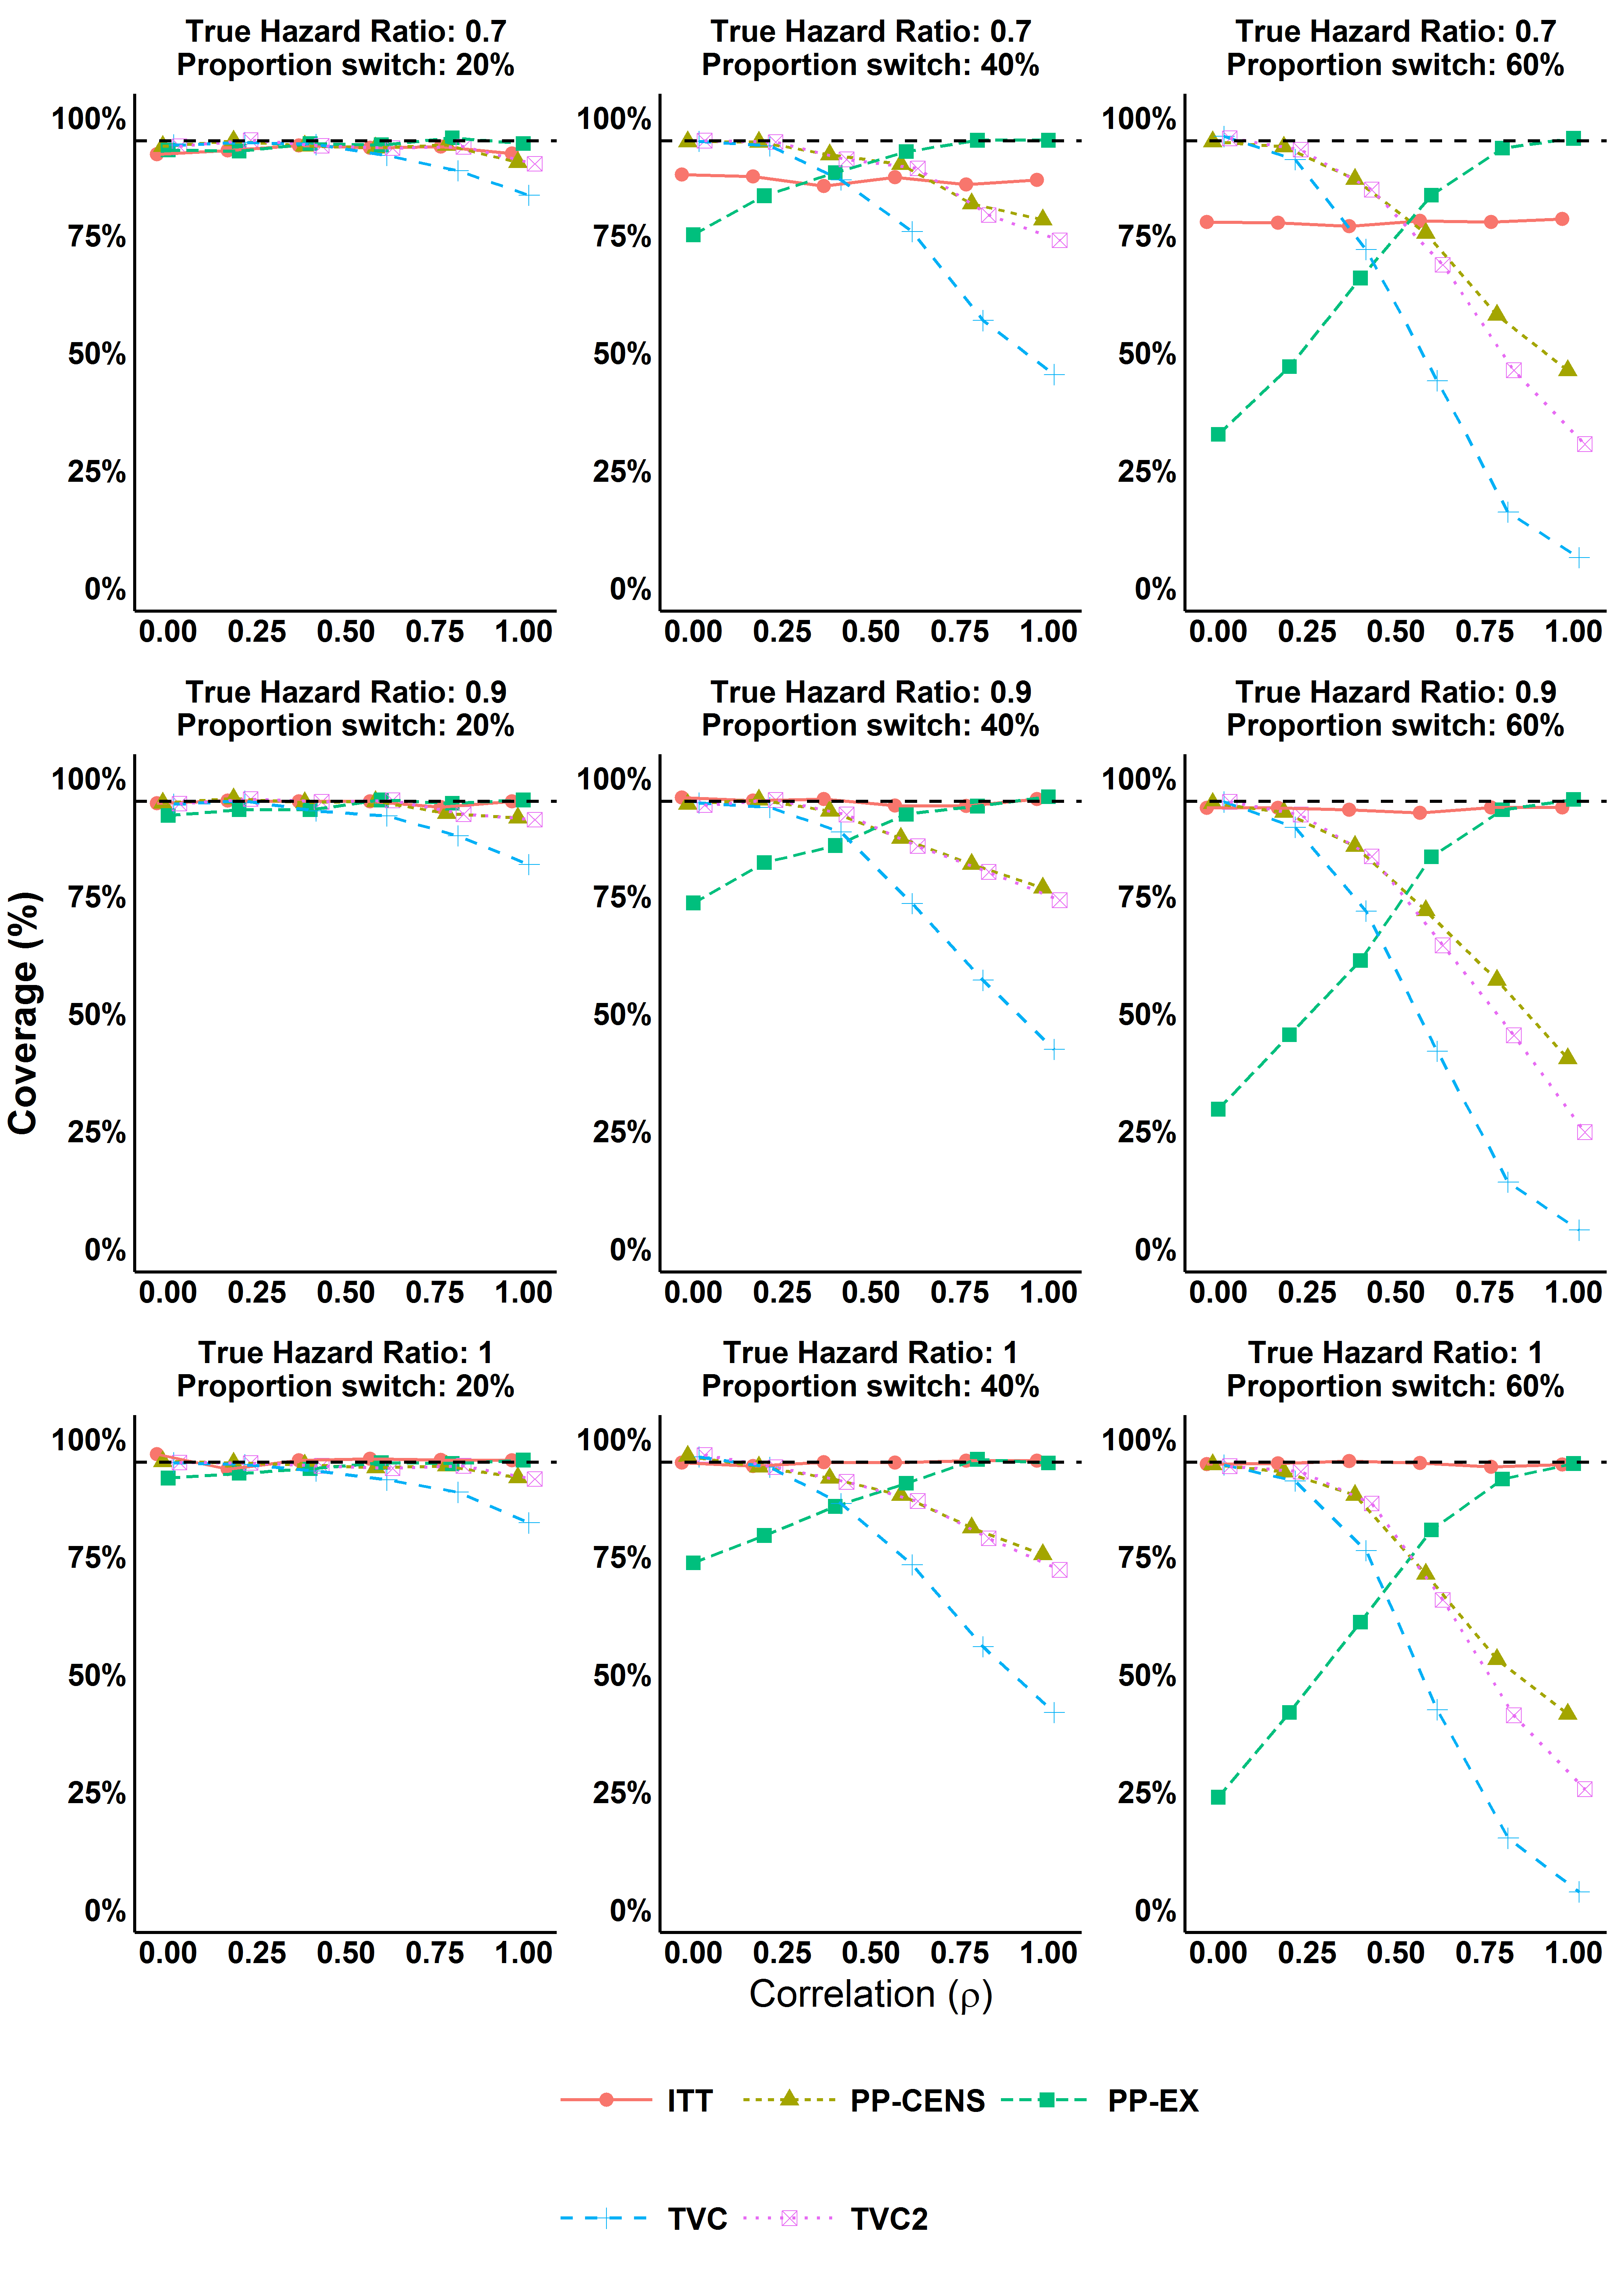
\includegraphics[width=13cm]{images/chap_sim2/simple_cov.png}
\caption{\label{F:chap_sim2:simp_cov} The coverage for each of the simple methods across all the scenarios. As with bias the performance of Censoring at switch (PP-CENS) and inclduing a time varying treatment covariate (TVC) is strongly related to correlation and very poor unless there is no correlation between TTP and OS. The method of excluding switchers (PP-EX) performs badly across every scenario except where the proportion of control patients switching is low.} 
\end{figure}

\begin{figure}[ht]
\centering
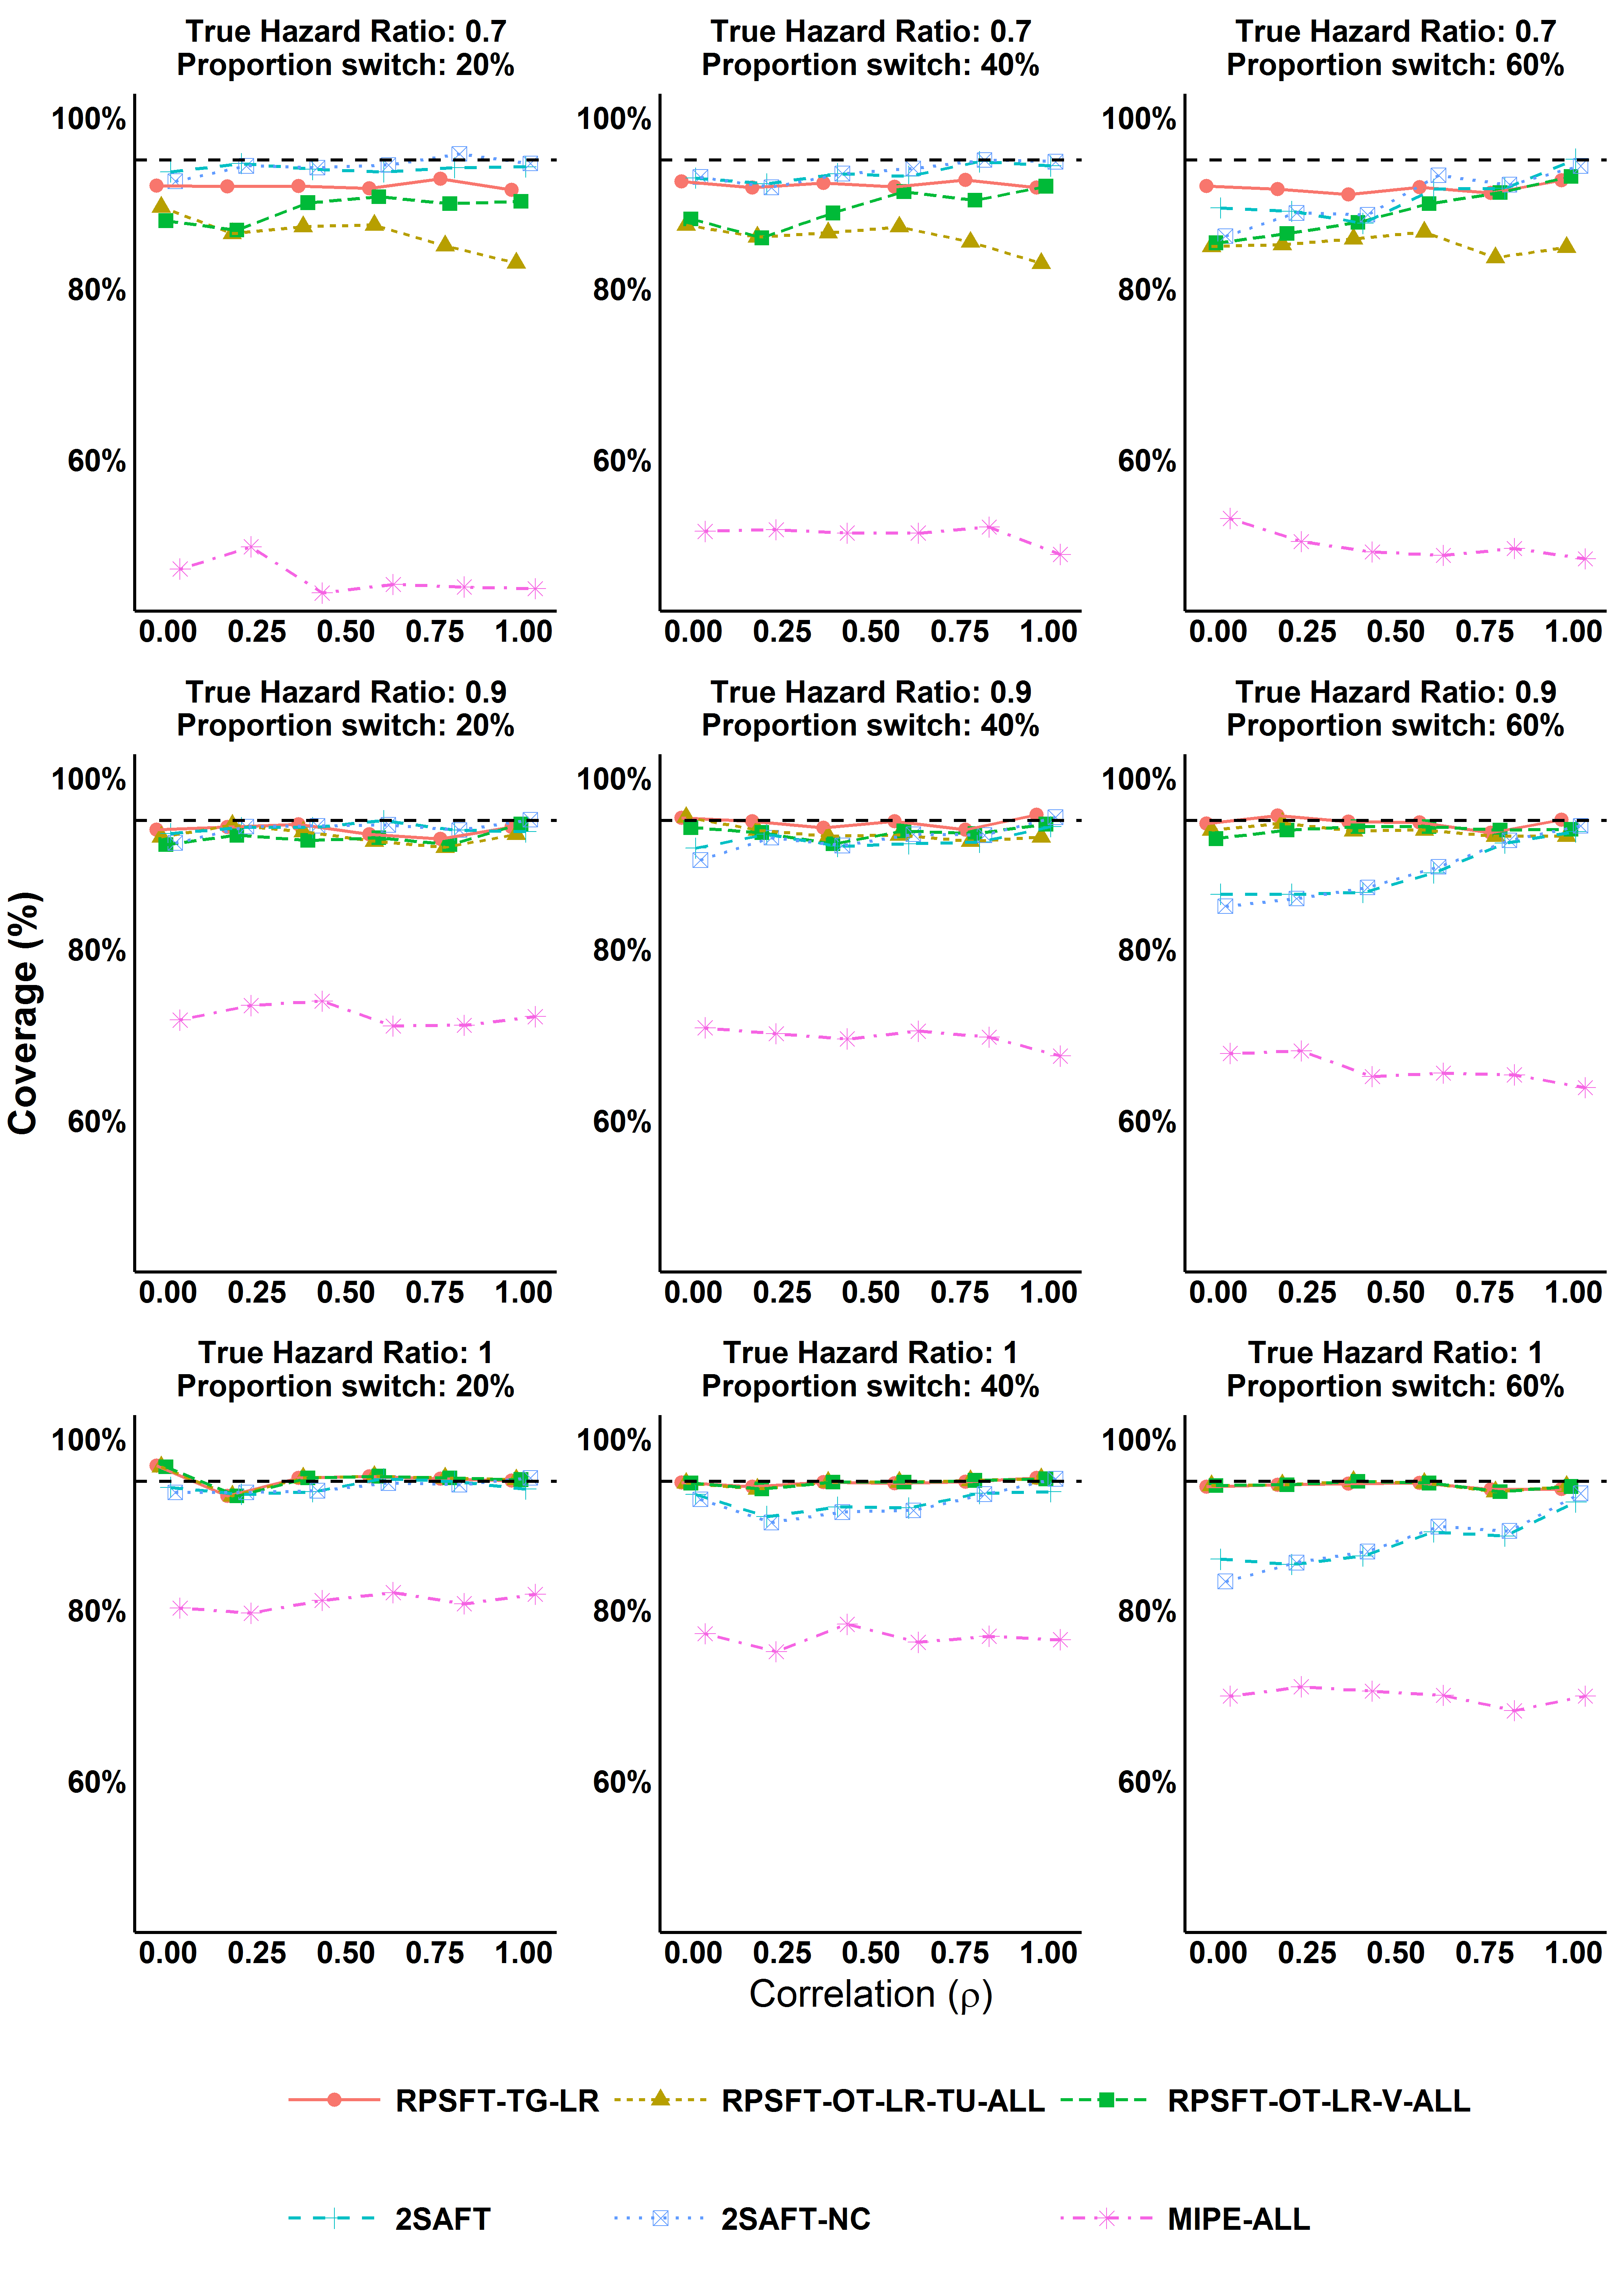
\includegraphics[width=13cm]{images/chap_sim2/complex_cov.png}
\caption{\label{F:chap_sim2:comp_cov} The coverage for each of the complex methods across all the scenarios. As expected bootstrapping of confidence intervals is needed for the MIPE and two-stage AFT (2SAFT) method with coverage poor particularly for scenarios where there is no treatment effect (True HR=1). The test-based correction proposed by \cite{White1999} performs reasonably but where there is a large treatment effect bootstrapping should be preferred.} 
\end{figure}

\clearpage 

\subsection{Convergence}
\begin{figure}[h!]
\centering
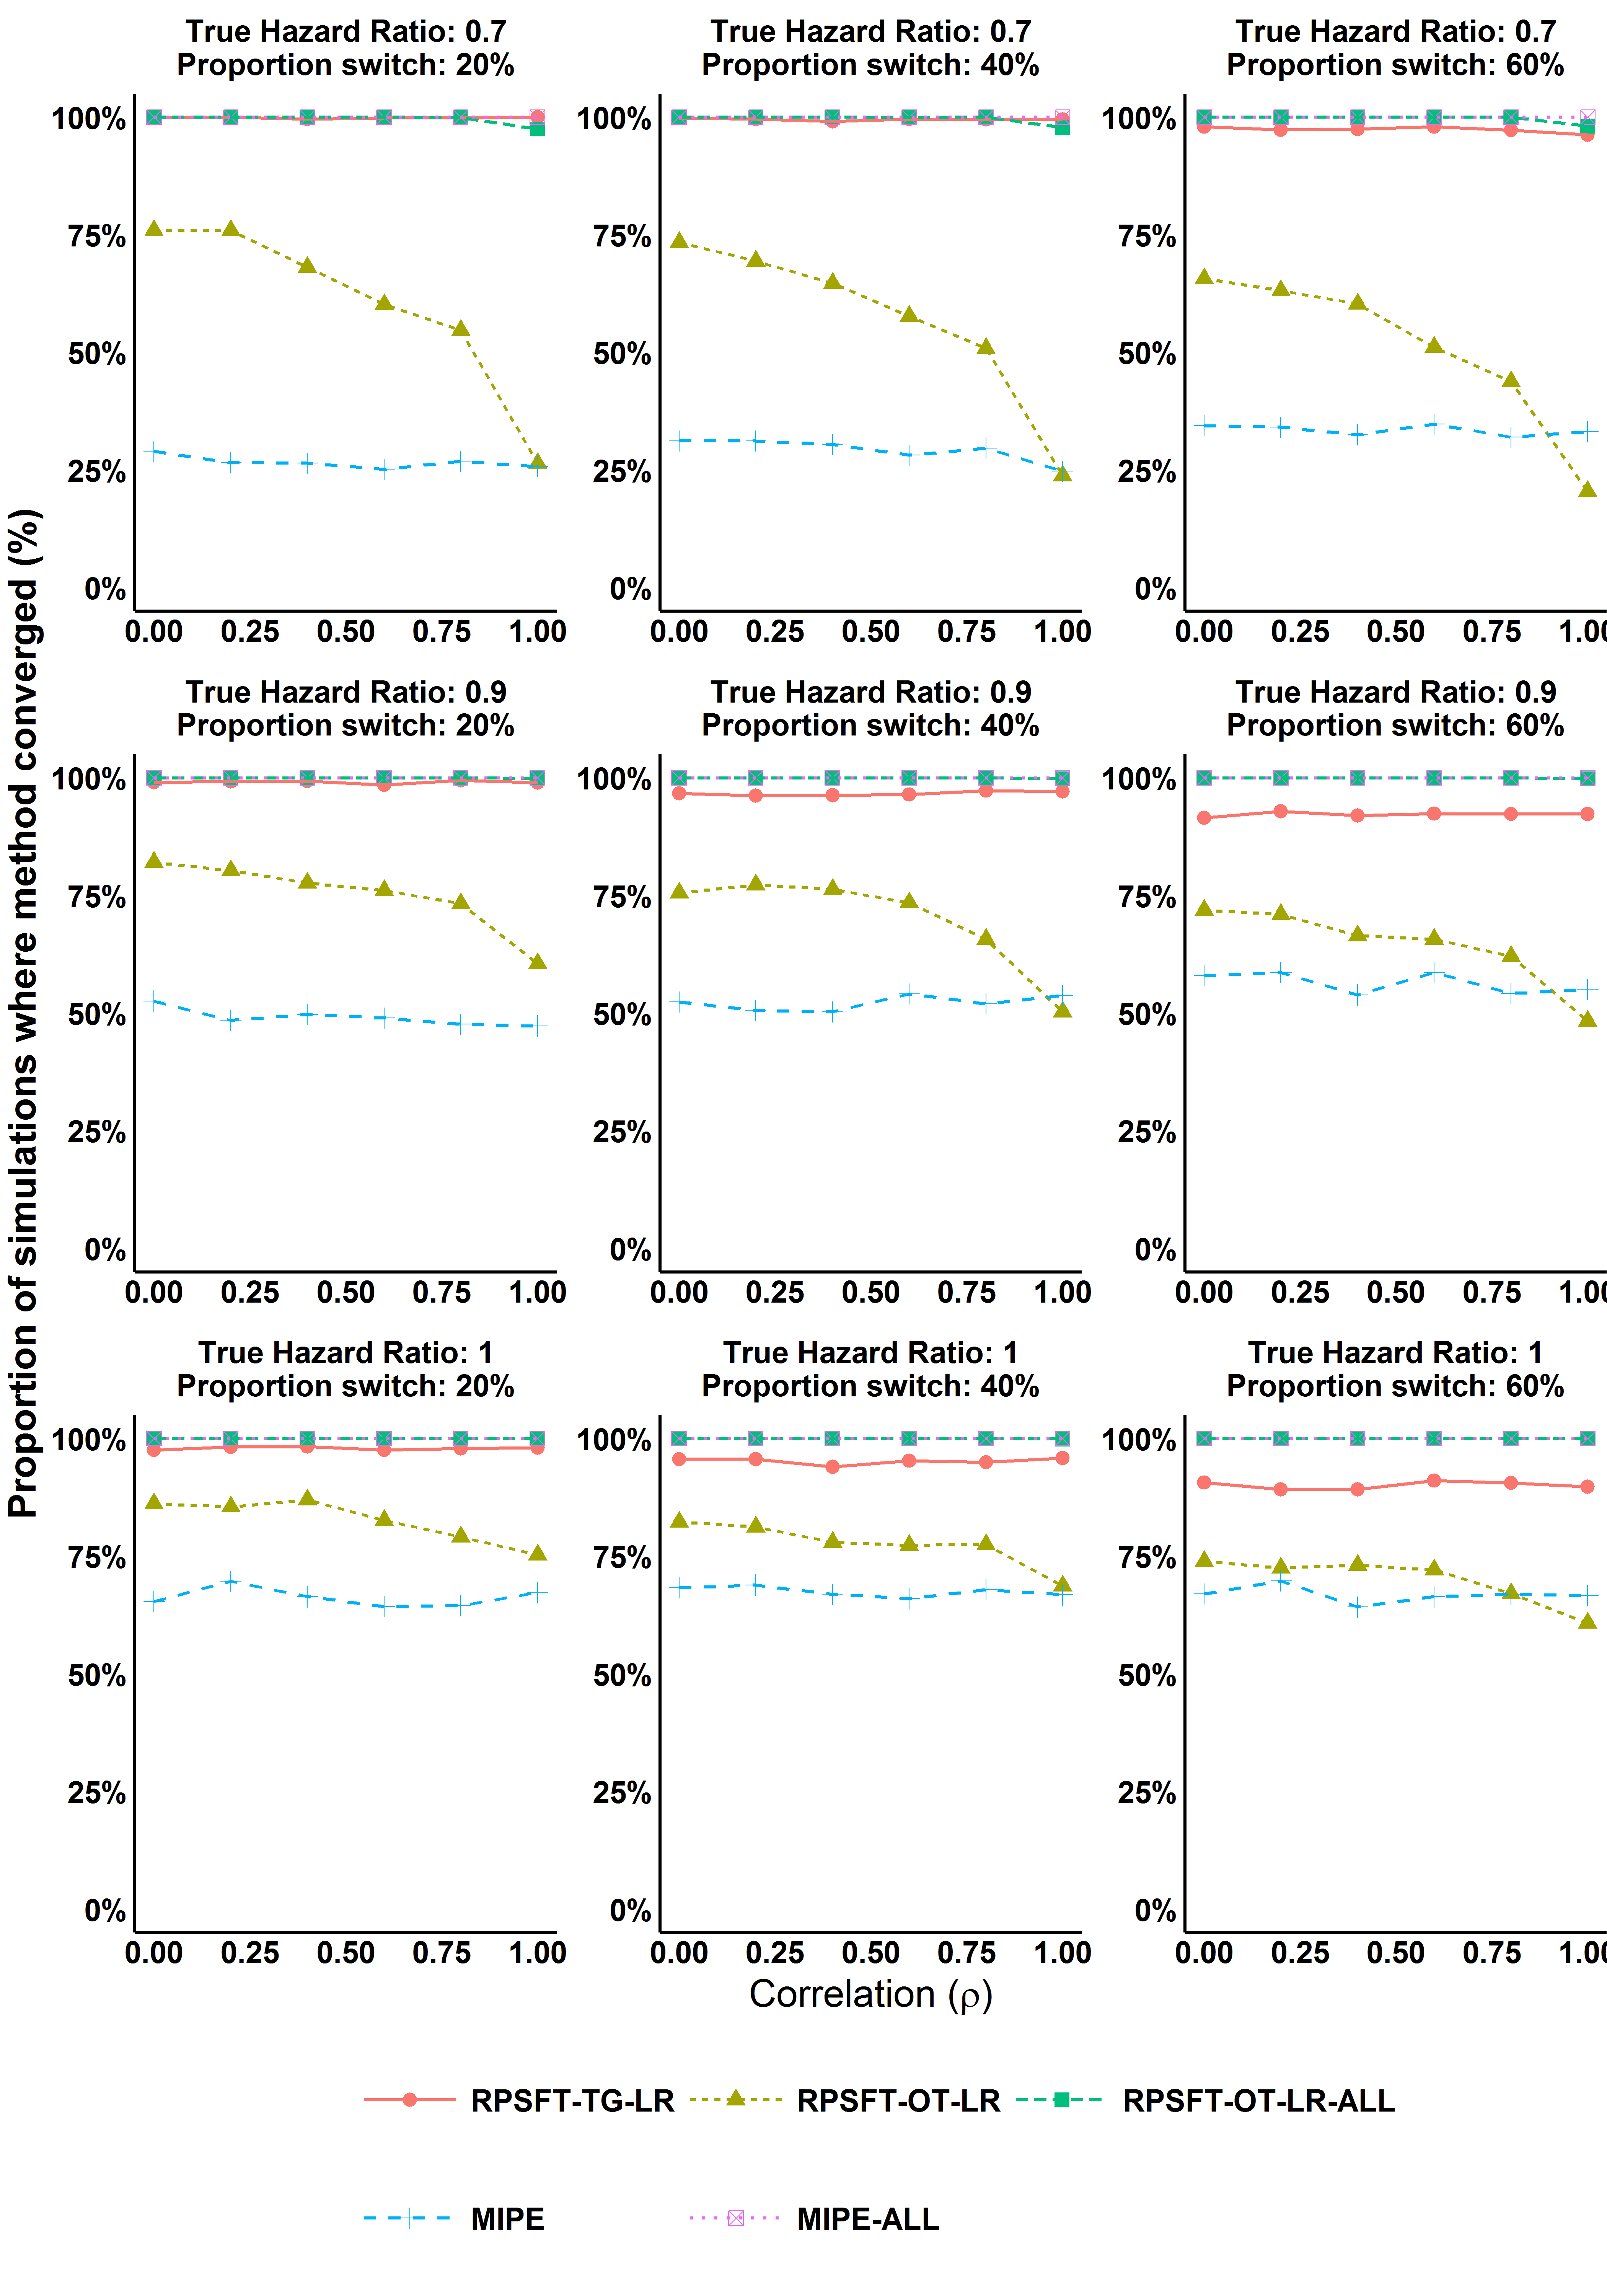
\includegraphics[width=13cm]{images/chap_sim2/complex_conv.png}
\caption{\label{F:chap_sim2:comp_conv} This figure shows the proportion of simulations where the complex methods rank-preserving failure time (RPSFT) and modified iterative parameter estimation (MIPE) converged to a unique solution. For the ``treatment group'' approach (RPSFT-LR-TG) convergence was high across all scenarios. For the ``on treatment'' approach (RPSFT-LR-OT) and MIPE the convergence was quite poor when the proportion of switch was high, the treatment effect was large or there was a large correlation between time to progression (TTP) and survival (OS). By using imputation approaches the convergence is improved to nearly 100\% for both RPSFT and MIPE (RPSFT-LR-OT-ALL, MIPE-ALL).}
\end{figure}

In Table \ref{T:chap_sim2:simres} and Figure \ref{F:chap_sim2:comp_conv} it can be seen that the complex methods sometimes fail to converge. The ``treatment group'' approach to rank-preserving failure time (RPSFT-LR-TG) modelling performed best with a lowest convergence across all scenarios of 89.2\%. This compares to the  ``on treatment'' approach (RPSFT-LR-OT) where for one scenario a unique solution was only found for 20.5\% of simulations and 24.8\% for the modified iterative parameter estimation (MIPE) method. When the imputations discussed in Section \ref{S:chap_sim2:convimp} the convergence can be increased dramatically for both approaches. Figure \ref{F:app_sim2:compA_bias} and Figure \ref{F:app_sim2:compA_cov} in Appendix \ref{A:sim2res} show that these imputations do not dramatically change the bias or affect the coverage of these methods and in the case of scenarios where convergence is very low they are beneficial. As the primary benefit of MIPE is an improved estimation algorithm this convergence performance is disappointing given the need to make additional assumptions over the RPSFT approach.


\clearpage

\section{Conclusion from simulation study 1}

In this simulation study the main parameter varied was the correlation between time to progression and overall survival. As observed in the simulation study from \cite{Morden2011} the ITT method underestimates the true treatment effect with the direction of bias being predictable regardless of correlation induced. Replicating the findings of \cite{Morden2011} it appears that both per-protocol analyses (censoring at crossover and excluding switchers) perform quite badly when a correlation is induced between time to progression and overall survival as the probability of switching is then dependent on prognosis. This is also the case of the approach of using a time-varying covariate in the cox model to estimate treatment effect. All of these methods appear to yield biased estimates when time to progression and overall survival times are correlated. 

As seen with the simulation study from \cite{Morden2011} the RPSFT method perform well regardless of correlation and flavour implemented. However, for MIPE the bias is in some scenarios larger than observed with the RPSFT which combined with the fact that convergence is worse than the ``treatment group'' approach to RPSFT and not consistently better than the ``on treatment'' approach means the value of this method seems limited given the need to make additional parametric assumptions.

The two-stage AFT method performs quite well in this simulation study showing similar bias to that seen with the ``treatment group'' approach to RPSFT when the model is correctly specified and recensoring is implemented. If the model is incorrectly specified by not including progression free-survival time then the bias is increased but is still lower than any of the simple methods considered here.

